\chapter{Cryptocurrency Wallets}
\label{ch:wallets}

Traditionally, you hold your cash in your wallet or banks store your fiat currency in an account in your name. The consensus is that you have access and can withdraw your currency at any time. In theory, this might sound correct, but the bank doesn't necessarily have your money. By converting fiat currency into cryptocurrencies, you can store your assets in such a way that only you can access them, you have full control at any time, without counterparty risk, because you  do not depend on anyone to get access.


\begin{quotation}
      \textit{\say{When you put your money in the bank, the bank becomes the owner of that money. With Bitcoin, you own your money. When the banks own that money, they spend it as they wish. When you own it, you spend it as you wish. It is censorship-resistant, and no one decides whether you can or cannot spend it and on what you will spend it on.}}
      \begin{flushright}
        \small{--- \textbf{Simon Dixon}}
      \end{flushright}
    
\end{quotation}

\begin{figure}
    \centering
    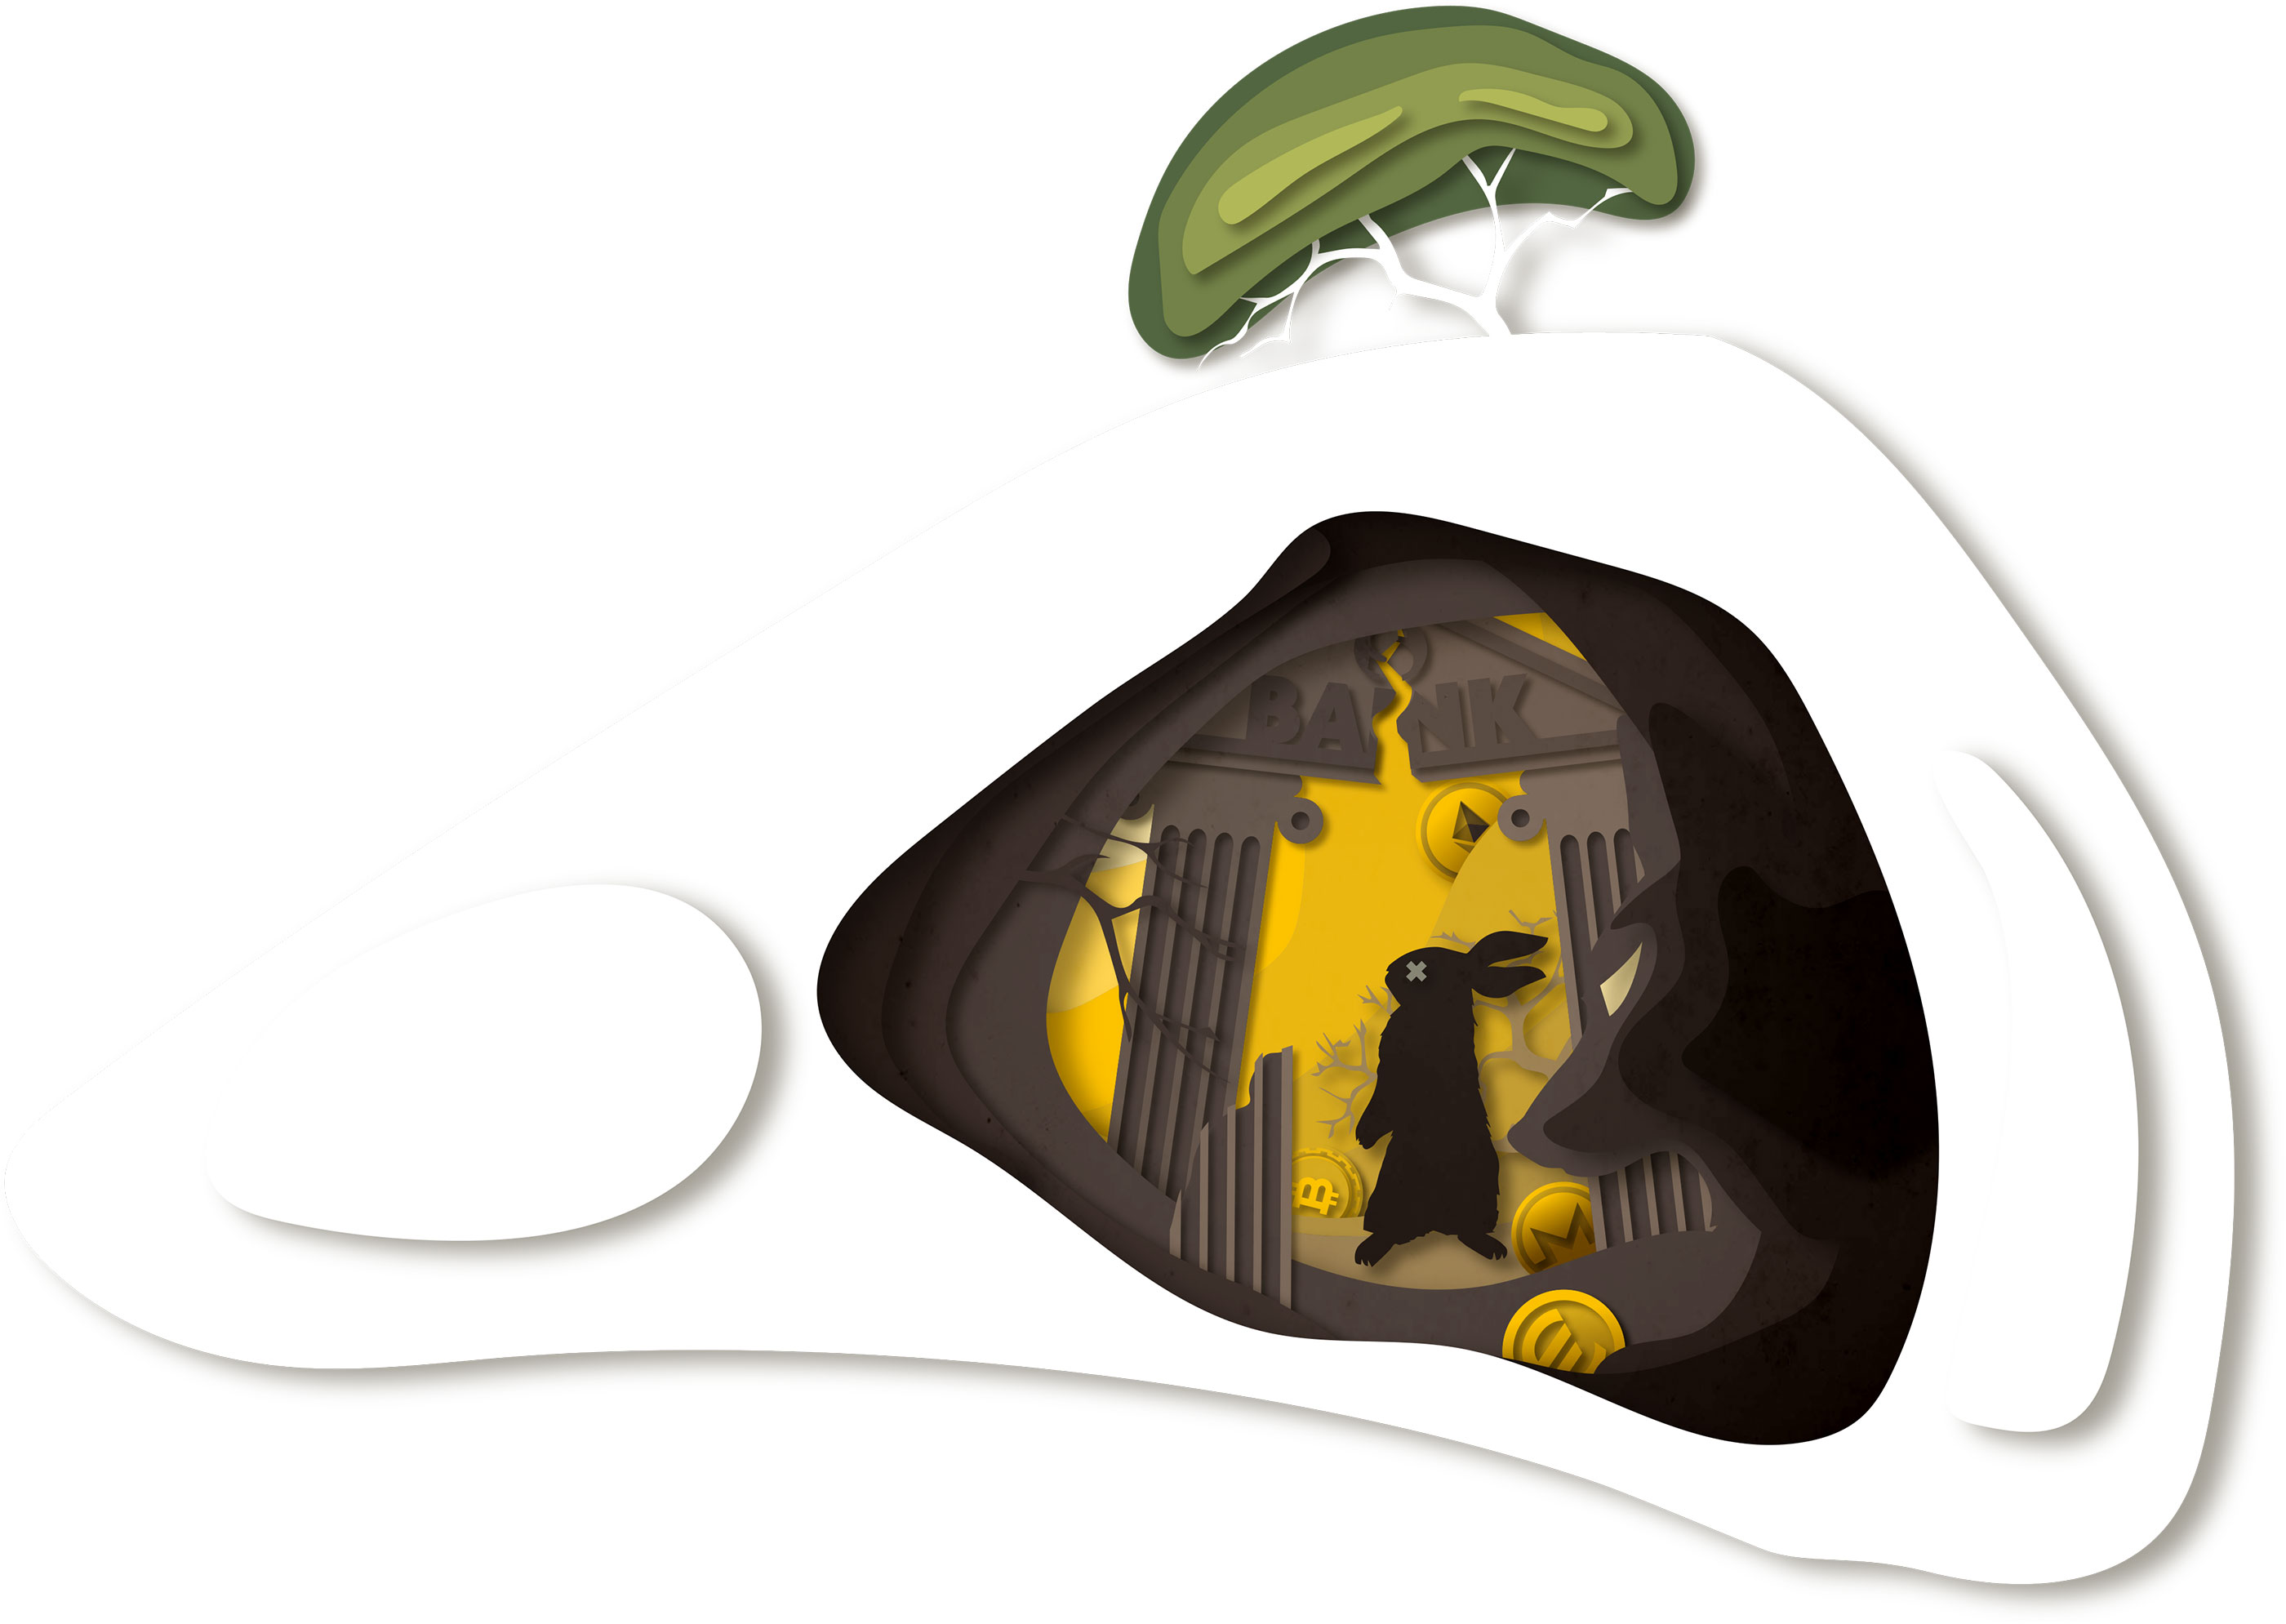
\includegraphics[width=\textwidth]{illustrations/resized_CRYPTO_KEY_1_PART_3.jpg}
\end{figure}

\section{Cryptocurrency wallets}
Cryptocurrency wallets are software programs that enable us to interface with the network (blockchain) to keep track of our transactions and assets. You can compare a cryptocurrency wallet with your bank account, a mailbox or an email address. You can interact with each of them if you have the required proof (respectively identity, key or password). If you want to own and use Bitcoin or any other cryptocurrency, you will need to have a wallet that supports the specific coin or token. 

\medskip
\begin{cryptobox}{\textbf{PLAY ON THE BLOCKCHAIN}}

    \say{A cryptocurrency wallet functions in the same way as your bank account in the sense that you can interface with the network and transact (deposit and withdraw) (crypto)currencies (\$, \pounds, \euro) to and from your bank account. With a cryptocurrency wallet, you manage your cryptocurrencies in the form of validated transactions on the blockchain. The wallet generates and stores private and public keys, interacts with the respective network (blockchain), and enables users to perform and sign transactions.} \footnote{Ethos (2018); \href{https://www.ethos.io/what-are-cryptocurrency-wallet-private-keys-addresses/}{What are Cryptocurrency Wallets, Private Keys and Addresses}.}

    \end{cryptobox}

\section{Different wallet types}
There are several types of wallets that provide different ways to store and access your digital currency. Wallets can be broken down into three distinct categories: software, hardware, and paper wallets. Software wallets could function on a desktop, online or mobile device and hardware wallets use software but fall in their category.

\medskip

\subsection{Hot storage versus cold storage wallets}
While you are reading about wallets, you might come across the terms \say{hot} wallets and \say{cold} wallets. All the different types of cryptocurrency wallets fall under either one of these two types.
In general, anything that is connected to the internet is less secure than something that is not. This is the difference between hot and cold wallets, with internet-connected wallets being hot and the other being cold. Online, desktop and mobile wallets are hot wallets, while hardware and paper wallets are cold wallets, also known as cold storage or hardware wallets (specialized USB enabled devices). Some might say that hardware wallets are prone to physical damage, loss or theft. However, the advantage is that they are far less likely to fall victim to hacking.

\subsection{Software wallets}
Software wallets can function on a desktop, online or on a mobile device.  Hardware wallets use their own software, although they fall under the hardware category because they are run as specialized USB devices.

\subsubsection{Desktop wallets (hot)} 
These are downloaded and installed on a PC or laptop. They are only accessible from the single computer on which they are downloaded. Desktop wallets offer one of the highest levels of security; however, if your computer is hacked or gets a virus, there is  a possibility  of losing all your funds.

\bigskip

\begin{borderbox}
    \centering
    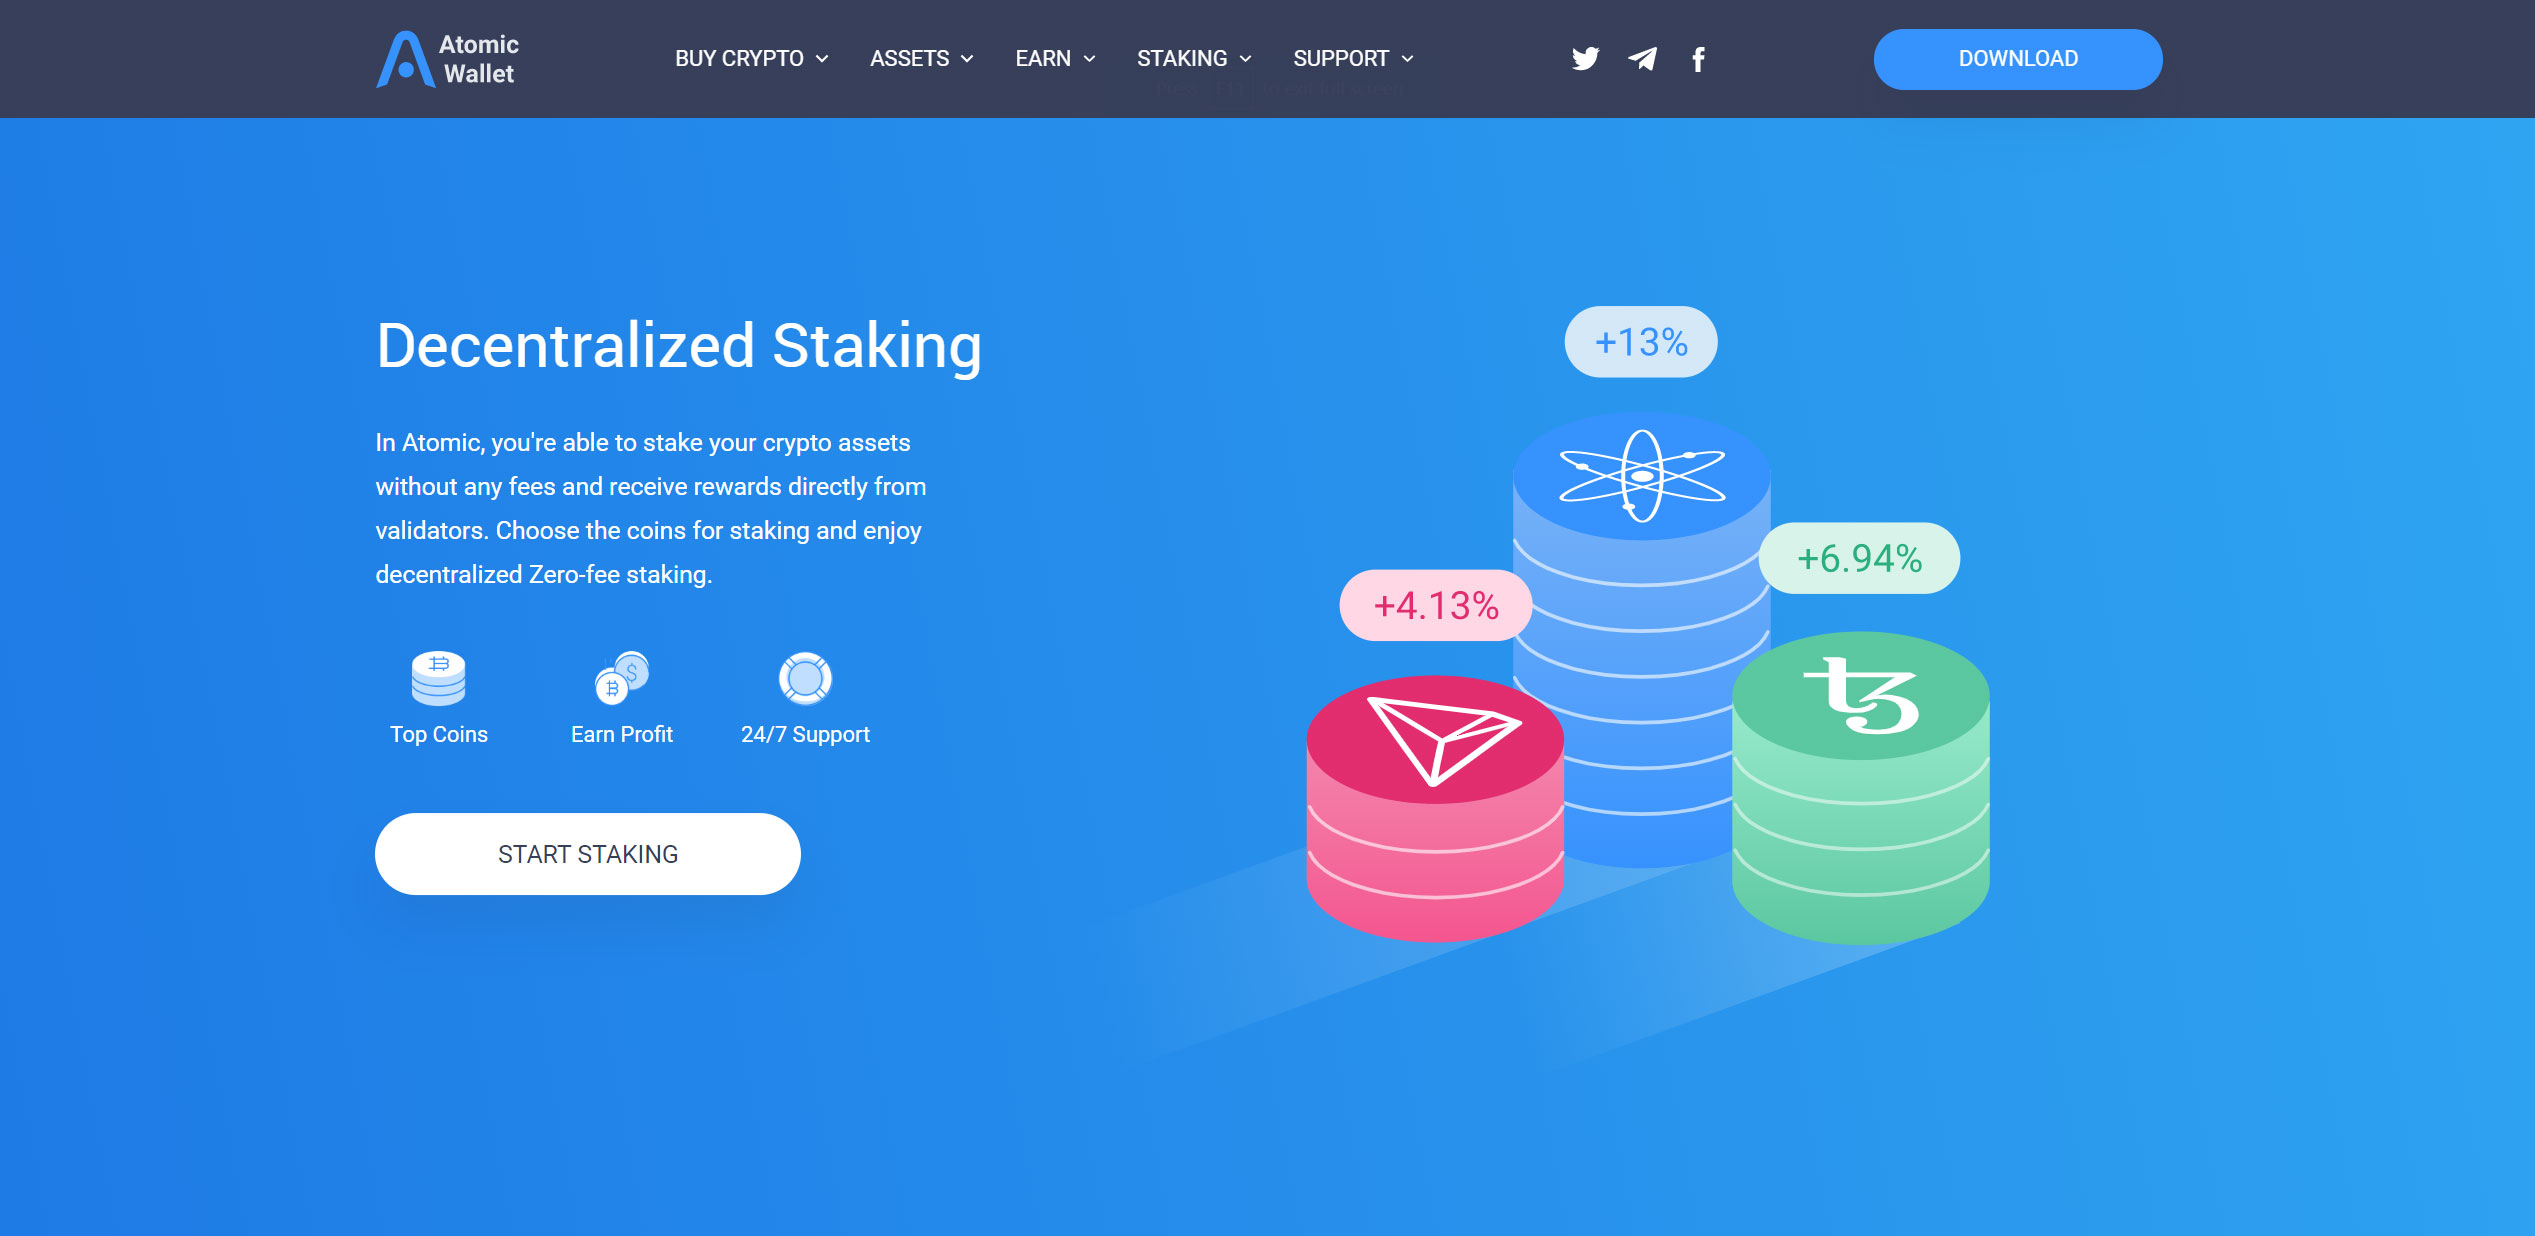
\includegraphics[width=\textwidth]{img/ch-wallets/atomic_wallet1.jpg}
\end{borderbox}
\medskip

\begin{tipbox}{\textbf{TIP}}
 Dekstop (software) wallets support many cryptocurrencies and are easy to use. Perfect for beginners.
\tcblower 
You can use \href{https://atomicwallet.io/}{Atomic Wallet} or \href{https://www.exodus.io/}{Exodus Wallet}.
\end{tipbox}\medskip

\subsubsection{Mobile wallets (hot)} 
These run on an app on your phone and are useful because they can be used anywhere, including retail stores. Mobile wallets are usually much smaller and simpler than desktop wallets because of the limited space available on a mobile.\medskip

\subsubsection{Web wallets or online wallets (hot++)}
Online wallets are the most notorious of all because you don't own your private keys. Exchange wallets are a prime example. Online wallets are accessible from any computing device and any location. While they are more convenient to access, online wallets store your private keys online, and if an exchange hosts the wallet, your keys are controlled by a (custodial) third party with centralized storage which makes them a huge target. These parties (usually large exchanges) are more prone and vulnerable to hacking and theft which is not uncommon as there is plenty of information available on the loss of user funds due to large scale security compromises. These were online "hot" exchange wallets where the user doesn't own his or her funds since he or she does not own the private keys.


\paragraph{Hosted wallets (custodial)}
The most notorious web wallets are the wallets that are managed by the various exchange platforms in a so-called \emph{online exchange wallet}. With these wallets, the user is not in possession of his or her private keys and the exchanges manage these for their users. Exchange account holders can log into their accounts with username and password combination, which are linked to the private keys of their stored cryptocurrency.

\paragraph{Non-hosted wallets}
Examples of non-hosted wallets are \href{https://www.myetherwallet.com}{MyEtherWallet} and \href{https://www.metamask.io}{MetaMask}.  Both enable users to fully control the cryptocurrencies themselves and are easy to manage and operate.

\bigskip
\begin{borderbox}
    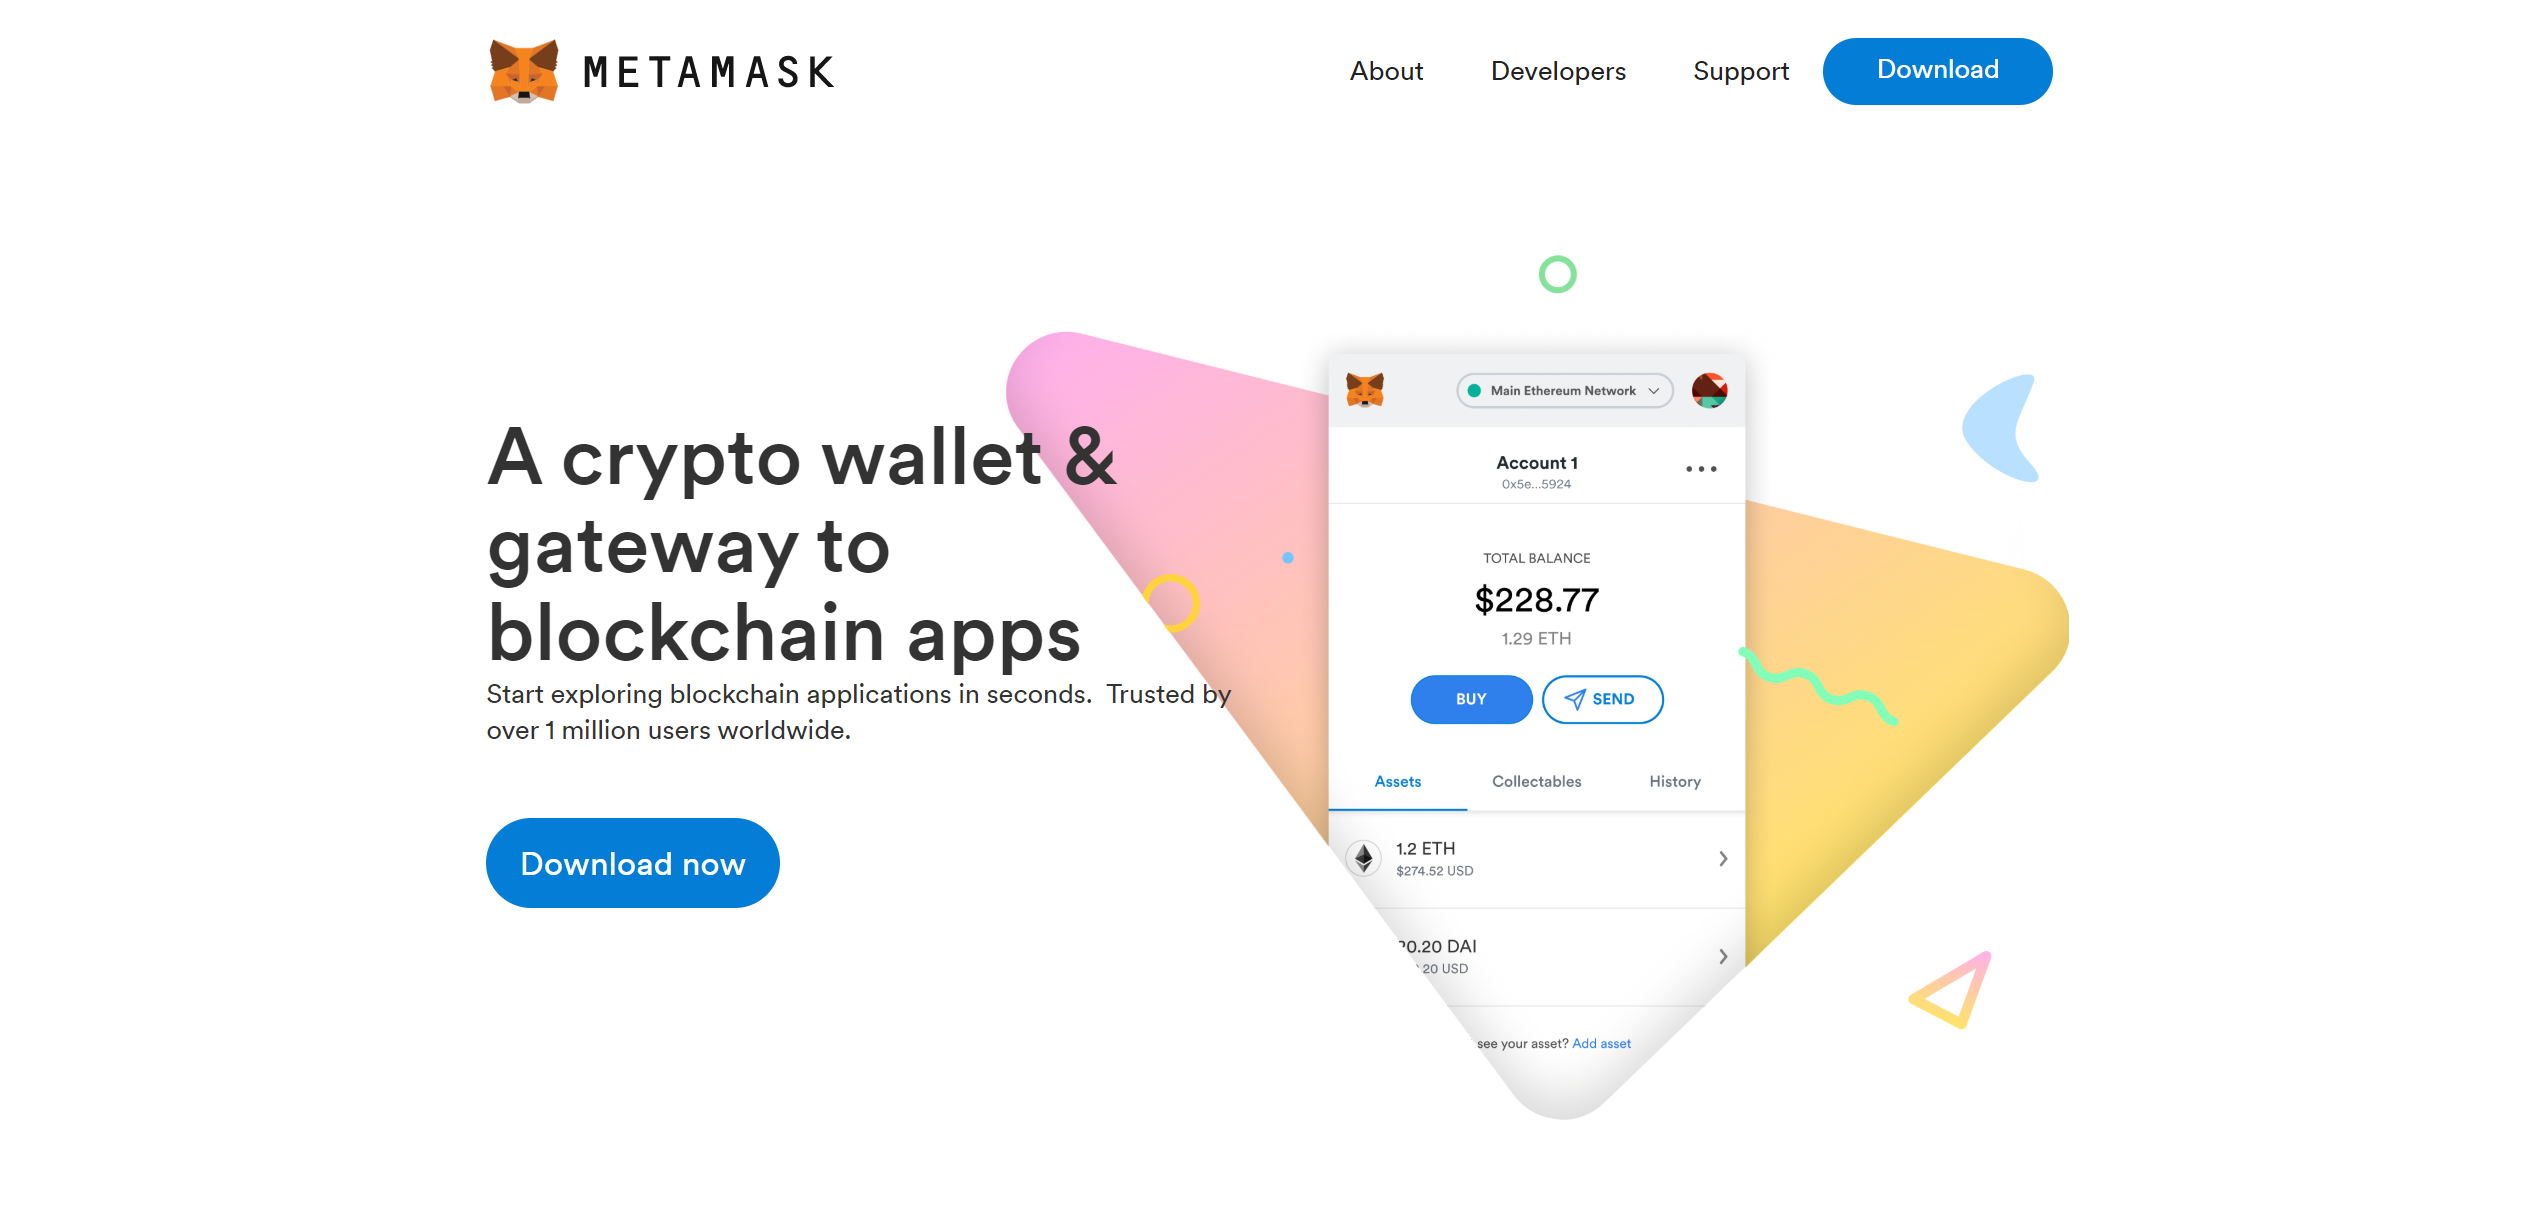
\includegraphics[width=\textwidth]{img/ch-wallets/metamask.png}
\end{borderbox}




\subsection{Hardware wallets (cold)} 
These differ from software wallets in that they store a user's private keys on a hardware device like a USB. Although hardware wallets make transactions online, they are stored offline, which delivers increased security. Hardware wallets can be compatible with several web interfaces and can support different cryptocurrencies; it just depends on which one you decide to use. What's more, making a transaction is easy. Users plug in their device to any internet-enabled computer or device, enter a pin, send currency and confirm. Hardware wallets make it possible to easily transact while also keeping your money offline and away from danger.

    \medskip
        \begin{tipbox}{\bf{TIP}}
        Hardware wallets store the private keys in a protected environment of the USB-device and the keys cannot be exported as text. In addition, hardware wallets are immune to computer viruses.
        \tcblower 
        For ultimate security, consider using a \href{https://shop.ledger.com/pages/ledger-nano-x?r=1849e3ffabd0}{Ledger} Hardware wallet.
    \end{tipbox}

\subsection{Paper wallets (cold)} 
These are easy to use and provide a very high level of security. While the term paper wallet can refer to a physical copy or printout of your public and private keys, it can also refer to a piece of software that is used to generate a pair of keys, which are then printed securely. Using a paper wallet is relatively straightforward. Transferring Bitcoin or any other currency to your paper wallet is accomplished by the transfer of funds from your software wallet to the public address shown on your paper wallet. Alternatively, if you want to withdraw or spend currency, all you need to do is transfer funds from your paper wallet to your software wallet. This process, often referred to as 'sweeping', can either be done manually by entering your private keys or by scanning the QR code on the paper wallet.

    \bigskip
    \begin{borderbox}
        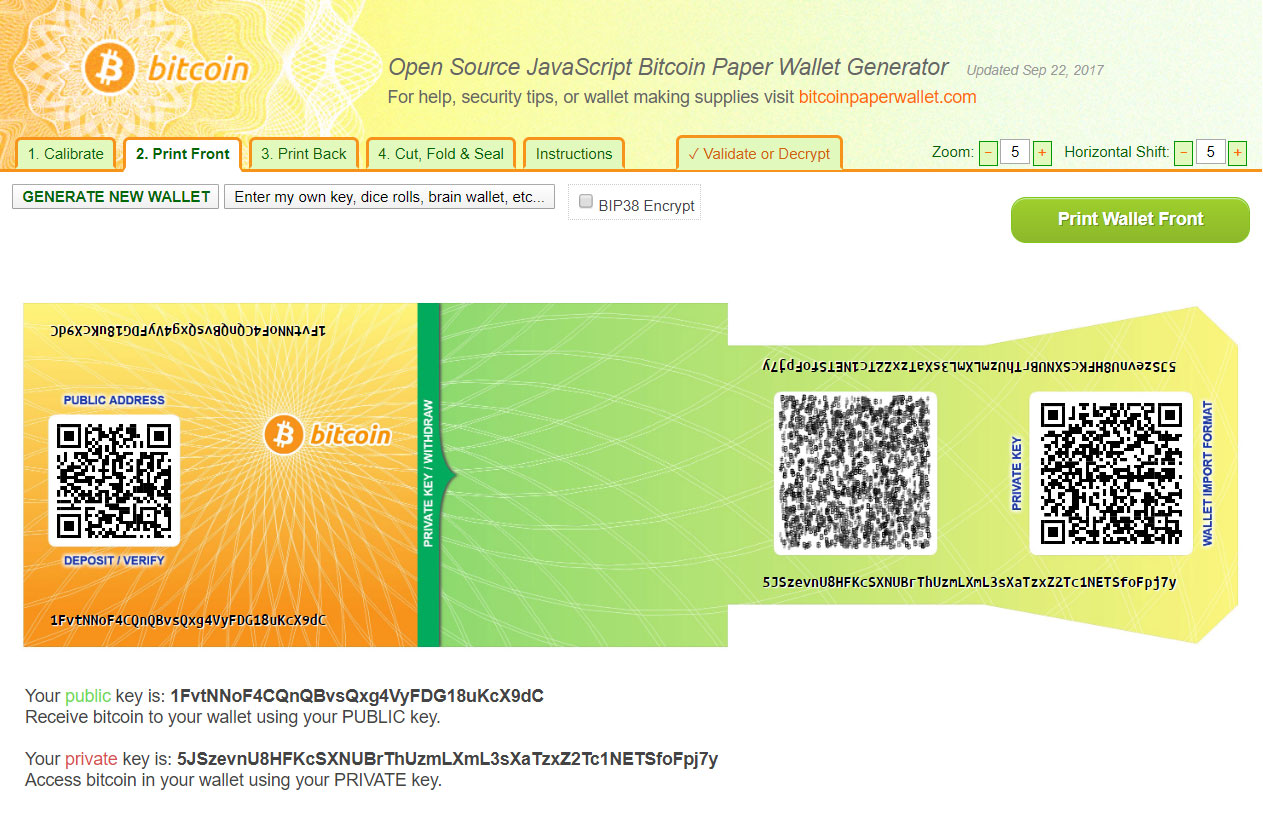
\includegraphics[width=\textwidth]{img/ch-wallets/paper-wallet-bitcoin.jpg}
    \end{borderbox}
    \medskip

    \begin{tipbox}{\textbf{TIP}}
    Use a cold wallet (hardware) to safely store the bulk of your crypto. Hot wallets (mobile, desktop or online) for that allocation of your portfolio with which you actively place buy and sell orders. 
    \end{tipbox}

\section{Important wallet considerations}
It is always a good idea to reduce potential risks by spreading around your assets if you have a lot of them. Take some digital 'cash' with you on a mobile wallet and keep the rest safe in (multiple) other locations. Don't keep all of your wealth in one place. 
\subsection{Risk of storing crypto on exchanges}
Security is a hot topic and a huge issue in the crypto environment and should never be taken lightly. On many centralized exchanges, you are not in control of your private key. Instead, exchanges let you log-in with a username and password combination. This implies that you do not truly own your assets, as the exchange "custodians" hold your private keys. Not owning your private keys means that you do not have full control over your funds.\medskip

Everyone knows exchanges are subject to attacks from malicious parties, trying to gain access to the funds of all users and the exchange reserves. For example, you sign up with an exchange, create an account protected with a password ( and 2FA) and the exchange gets hacked or otherwise compromised; you might well lose your investments since the hackers now have access to the private keys of registered users of the exchange. Now the exchange functions precisely the same as a regular bank. 
\medskip

\begin{quotation}

      \textit{\say{Not your keys, not your Bitcoin.}}
      \begin{flushright}
        \small{--- \textbf{proofofkeys.com}}
      \end{flushright}
    
\end{quotation}

\subsection{Security and technical complexity}

Keep in mind that a safer and more secure wallet adds more layers of technological sophistication. This complexity, in itself, imposes additional risks if you do not know precisely what you are doing. It is a lot easier to run a wallet on your mobile phone or desktop with a simple PIN or password, then it is to run dedicated cold storage or multi-signature wallet. People who overextend (because they aim for higher security) might just as well lose their funds because they underperform on execution and handling of these more complicated systems. Assessing what an acceptable level of risk for your specific situation and circumstances is based on your commitment and invested funds.\medskip

\subsection*{Which wallet is best for me?}

There are a lot of different wallets available and more diverse and advanced wallets are being launched frequently. Before selecting a wallet, you should think carefully about how you intend to use it. Do you need a wallet for everyday purchases, or do you need a wallet where you can actively trade? Should you also have a dedicated wallet that functions as an offline vault for your long term investments? Are you planning on using a host of cryptocurrencies, or only Bitcoin? Do you require access to your digital wallet from multiple devices or just your mobile phone? 

    \bigskip
    \begin{tipbox}{\textbf{TIP}}
    Take the time to assess your requirements and only then decide on the most suitable wallet(s) for you. You cannot go wrong with the wallets we recommend, with which you will have a complete cryptocurrency set-up. 
    \end{tipbox}

\section{Combinations of cryptocurrency wallets}
In general, try to reduce potential risks by spreading around your assets if you have a considerable amount invested. When you diversify, you aim to manage your risk by spreading out your funds. You can, of course, expand and diversify both within and among different asset classes. But when it comes to cryptocurrencies, you can take any number of assets with you on a mobile wallet and store the rest safely on (multiple) other locations. For instance, you would have registered at one broker exchange (to convert your fiat to crypto) and at another trading exchange (where you trade crypto to crypto). You might also have a dedicated hardware wallet to store the majority of your assets offline and have a small portion on a wallet on your phone to be able to take with you for easy access and liquidity purposes. Take some time to assess your requirements and only then decide on the most suitable wallet(s) for you. 

\begin{table}

\centering

\caption[A selection of cryptocurrency wallets]{A selection of popular cryptocurrency wallets for your review. Exchange wallets are not considered, but some of these are highlighted in \cref{ch:exchanges}.}
\begin{tabular}{llll} 
\toprule

\textbf{Wallet} & \textbf{Support} & \textbf{Platform} & \textbf{URL }\\
\midrule

Ledger          & multi    & hardware   & \href{https://shop.ledger.com/pages/ledger-nano-x?r=1849e3ffabd0}{ledger.com}\\
KeepKey         & multi    & hardware   & \href{http://lddy.no/aczp}{shapeshift.io}\\
Trezor          & multi    & hardware   & \href{https://shop.trezor.io/?offer_id=10&aff_id=3118}{trezor.io}\\
Electrum        & BTC      & desktop    & \href{https://electrum.org/#home}{electrum.org}\\
Atomic          & multi    & desktop    & \href{https://atomicwallet.io/}{atomicwallet.io}\\       
MEW             & ETH      & web        & \href{https://www.myetherwallet.com/}{myetherwallet.com}\\
MetaMask        & ETH      & web        & \href{https://metamask.io/}{metamask.io}\\
Exodus          & multi    & desktop    & \href{https://exodus.io/}{exodus.io}\\
Ethos           & multi    & mobiel     & \href{https://www.ethos.io/universal-wallet/}{ethos.io}\\
Abra            & multi    & mobiel     & \href{https://www.abra.com/}{abra.com}\\
Edge            & multi    & mobiel     & \href{https://edge.app/}{edge.app}\\
Changelly       & multi    & web        & \href{https://changelly.com/}{changelly.com}\\ 
ShapeShift      & multi    & web        & \href{https://shapeshift.com/#top}{shapeshift.com}\\




\bottomrule
\end{tabular}
\label{tab:walletoverview}
\end{table}








